\documentclass{solitairemiya-art}

\usepackage{graphicx}
\usepackage{amsmath}
\usepackage{amssymb}
\usepackage{booktabs}
\usepackage{multirow}
\usepackage{array}

\title{二进制与随机逻辑混合计算}
\author{Hongge Li, IEEE会员，以及 Yuhao Chen, IEEE研究生会员}

\begin{document}

\maketitle

\begin{abstract}
二进制逻辑广泛应用于数字信号处理和计算机系统，因其可直接在CMOS电路中实现. 随机逻辑采用特殊的数据表示方式，以逻辑电平为ON的概率表示数据. 随机逻辑计算是基于随机比特流而非二进制数的计算类型. 本文提出一种二进制逻辑与随机逻辑的混合计算系统，称为混合逻辑计算. 文中讨论了混合逻辑电路的生成方法，并分析其特性. 

\noindent\textbf{关键词：}现场可编程门阵列(FPGA)，混合逻辑计算，低延迟，随机计算(SC)
\end{abstract}

\section{引言}

随机逻辑的特性一直是学术界的研究热点. 随机逻辑本质上是一个基于概率与均值的数学问题，利用简单逻辑电路即可实现具有特殊性质的随机逻辑功能，从而替代基于二进制逻辑的复杂电路. 另一方面，在二进制逻辑（布尔代数）中，系统任意节点的变量仅能取两个值之一，记为0或1. 

随着计算规模增大，传统数字计算的功耗需求随之增加，导致计算规模与求解速度之间需要权衡. 为此，研究者提出了一种新的数据处理系统——随机计算（SC），该系统最大化利用各逻辑门进行计算，并以分布式方式在空间和时间上执行运算. 

二进制逻辑在执行数字计算时具有显著的速度优势. SC是由Gaines于1969年提出的一种重要脉冲计算方法[1]. 在SC范式中，计算基于随机比特流（SB）而非二进制数（BN）进行. SB通过比特流中"1"的出现概率表示数值，该概率基于累积时间计算[1],[2]. SC所需的计算能力完全分布于低成本的逻辑门中. 二进制逻辑电路采用高效的数据编码方式，仅需$\log_2 N$个有序二进制电平. 相反，SC是数据表示效率最低的方式，需要$N^2$个无序二进制电平[1]. 然而，传统SC以牺牲效率为代价，换取了大量硬件资源和功耗的节省. 

\begin{figure}[htbp]
\centering
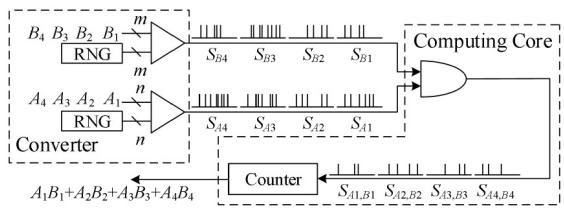
\includegraphics[width=0.8\linewidth]{images/095e8cba1e8ee880128a0ef6072ed1b6b4847435387346cfef71f37f9cd1e5f8.jpg}
\caption{基于SB的经典SC}
\label{fig:1}
\end{figure}

在SC范式中，数字计算基于SB而非BN进行，这在处理复杂函数时具有显著的硬件开销优势. SC已广泛应用于多个领域[2],[3]，包括图像处理[4]、通信编码[5]、神经网络[6]和深度学习[7]. Sim等人提出了新的乘法方法，用于缩短流长度并优化高延迟问题. Najafi和Lilja[8]提出了确定性方法以实现精确计算. Parhi[9]提出了单极性与双极性混合格式，以获得更好的能效. Liu和Han[10]采用Sobol序列优化精度不足的问题. Canals等人[11]提出了一种新的编码方法，以分数形式用两组SB表示一个值，将脉冲表示范围扩展至整个实数轴. 

传统SC的高延迟本质上源于1比特随机流较低的信息携带能力. 当随机逻辑的比特流长度为$N$时，其仅能表示$N$个不同的数值. 显然，比特流的信息携带效率低于BN. 为提高SC编码效率，研究者尝试了多种方法，如使用多比特流缩短延迟[12],[13]，或采用温度计编码器[14]. 

尽管SC在硬件开销和噪声容限方面具有优势，但高延迟和低精度仍是SC硬件电路设计面临的主要挑战. 为解决这些根本性问题，本文提出了一种新的计算方法. 主要贡献如下：
\begin{enumerate}
    \item 提出了二进制逻辑和随机逻辑的混合逻辑计算，用于混合逻辑SC(HSC). 
    \item 讨论了混合、随机和二进制逻辑的性质和关系. 
    \item 设计了乘法器、加法器、除法器以及BN和SB转换器的混合逻辑电路. 
\end{enumerate}

\section{随机计算}

\subsection{现有SC方法}

基于随机比特流的经典SC乘法[1]如图\ref{fig:1}所示. 随机比特流生成器由随机数生成器（RNG）和比较器组成. 通过比特流生成器，$A$和$B$分别被转换为随机比特流$S_A$和$S_B$. 两个流为"1"的概率分别为$P(S_A) = A/2^n$和$P(S_B) = B/2^m$. 经"AND"门后得到新的随机比特流$S_{A,B}$. 输出流为"1"的概率为$P(S_{A,B}) = P(S_A)P(S_B) = AB/2^{n+m}$，实现了两个输入流$S_A$和$S_B$的乘法. 计数器逐个累加四个随机流$S_{A1,B1}$至$S_{A4,B4}$，以获得$A_1B_1 + A_2B_2 + A_3B_3 + A_4B_4$的完整结果. 

SC结果可能存在误差的原因如下. 首先，两个输入流须相互独立；否则$P(S_{A,B}) = P(S_A)P(S_B)$不成立. 其次，随机流本质上是$N_F$重伯努利试验的结果，流中"1"的数量服从二项分布[11]. SB的长度随所需分辨率呈指数增长. 例如，要获得具有8位分辨率的流概率，使用经典SC须观察至少$2^{16}$比特的流长度[15]. 

\subsection{随机与二进制混合逻辑}

SC通常以流中"1"的概率表示数值. 设$x(1), x(2), \ldots, x(N)$为该流. 比特流中的每个$x(i)$由离散随机变量$X$生成，其概率分布为$P(X=1) = p$和$P(X=0) = 1-p$，其中$p$为概率值. 根据已有研究中期望的定义，$X$的期望可由下式求得[17]：
\begin{equation}
E[X] = 1 \cdot p + 0 \cdot (1-p) = p.
\label{eq:1}
\end{equation}

由(1)可知，SC亦可理解为使用离散随机变量$X$作为信号源生成随机流，且$E[X]$表示该流的值. 由于在传统SC中$X$取值为1或0，故随机脉冲为1比特流. 

按上述方式理解，离散随机变量的取值范围可进一步扩展，而非局限于1比特流. 因此，SC可扩展为使用多比特流替代1比特流. 图\ref{fig:2}和图\ref{fig:3}展示了在2比特流上进行计算的示例. 由于这种新的随机流兼具传统随机逻辑与二进制逻辑的特性，本文将新方法称为随机与二进制的混合逻辑计算，并将多比特随机流称为混合流. 

\begin{figure}[htbp]
\centering
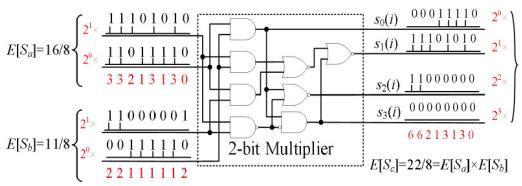
\includegraphics[width=0.8\linewidth]{images/143ce7be794b95afb5a8e01d5237b2ee955b69f635a55e03c96163dd13761bfe.jpg}
\caption{HSC的乘法}
\label{fig:2}
\end{figure}

\begin{figure}[htbp]
\centering
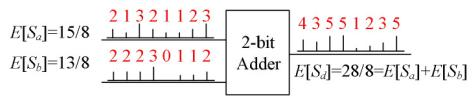
\includegraphics[width=0.8\linewidth]{images/27331e1b728b00a30ec29ce053ccb6773ae29b56081dea78cda635e712b7dc82.jpg}
\caption{HSC的加法}
\label{fig:3}
\end{figure}

\textbf{1) 乘法和加法：}将混合流$s_a(i)$和$s_b(i)$逐元素相乘，可得新的混合流$s_c(i)$
\begin{equation}
s_c(i) = s_a(i)s_b(i).
\label{eq:2}
\end{equation}

根据概率理论，若$s_a(i)$和$s_b(i)$相互独立，则$s_c(i)$的期望为$E[S_a]$与$E[S_b]$之积，如(3)所示. 因此，(2)实现了两个混合流的乘法运算. 
\begin{equation}
E[S_c] = E[S_aS_b] = E[S_a]E[S_b].
\label{eq:3}
\end{equation}

将两个混合流$s_a(i)$和$s_b(i)$逐元素相加，可得新的混合流$s_d(i)$
\begin{equation}
s_d(i) = s_a(i) + s_b(i).
\label{eq:4}
\end{equation}

根据概率定理，$s_d(i)$的期望等于$E[S_a] + E[S_b]$，如(5)所示. 因此，(4)实现了两个混合流的加法运算. 
\begin{equation}
E[S_d] = E[S_a + S_b] = E[S_a] + E[S_b].
\label{eq:5}
\end{equation}

下面以图\ref{fig:2}为例说明细节. 首先将BN 16和11缩放至$[0, 2^2-1]$范围，以满足2比特混合流的表示范围. 由此，2比特流以$E[S_a] = 16/8$和$E[S_b] = 11/8$编码，分别表示16和11. 采用这种混合逻辑，可使用2比特乘法器实现$n$比特$(n \geq 2)$二进制乘法，如图\ref{fig:2}所示；使用2比特加法器实现$n$比特$(n \geq 2)$加法，如图\ref{fig:3}所示. 

混合逻辑流不仅由2比特组成. 当使用$m$比特混合流表示$n$比特二进制数据$(m \leq n)$时，可以使用$m$比特乘法器进行$n$比特二进制乘法. 

\textbf{2) 除法：}图\ref{fig:4}(a)展示了HSC除法电路结构. 其中，$s_a(i)$和$s_b(i)$为输入混合流，$i = 0, 1, \ldots, N-1$；除法结果$s_c(i)$亦为混合流. 计数器用于计算$\sum_{i=1}^{n}|\overline{s_a}(i) - s_c(i)s_b(i)|$. 当计数器的期望等于0时，$E[S_cS_b] = E[S_a]$成立. 在此条件下，若$S_c$和$S_b$相互独立，则有$E[S_c]E[S_b] = E[S_a]$. 因此，当计数器趋近于0时，$s_c(i)$即趋近于除法结果. 将计数器和$s_c(0)$的初始值均设为零，并使用RNG控制$s_c(i)$的值：当计数器$>0$时，$s_c(i) = \text{RNG}$；当计数器$<0$时，$s_c(i) = 0$. 除法电路的精度测试如图\ref{fig:4}(b)所示，当$E[S_a] = 3$且$n = m = l = 3$时，$E[S_c] = 3/E[S_b]$. 除法电路的数据流示例如图\ref{fig:4}(c)所示. 

\begin{figure}[htbp]
\centering
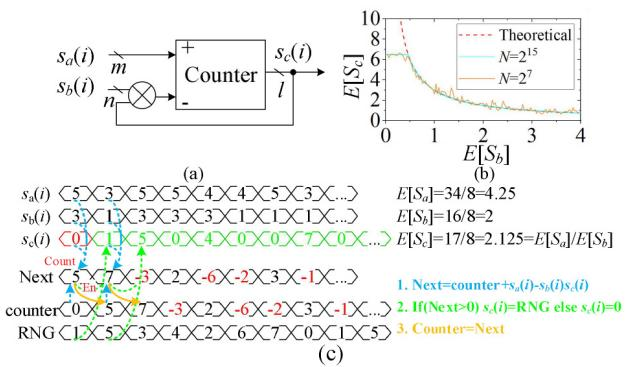
\includegraphics[width=0.9\linewidth]{images/52628885b9c1a8f8e3a8924c8686f97957da5de167ff9404291eb97f0e6cea51.jpg}
\caption{HSC的除法. (a)除法计算电路. (b)除法电路的精度评估，$E[S_c] = 3/E[S_b]$. (c)除法电路示例. }
\label{fig:4}
\end{figure}

\textbf{3) BN-SB转换器：}本文提出了两种类型的BN-SB电路，即A型和B型，如图\ref{fig:5}所示. BN-SB（A型）以一个BN $x$（n比特）作为输入来编码多比特流. 例如，图\ref{fig:5}(a)展示了$m$比特随机流的编码过程，其中$x_i$表示$x$的第i位. $x$的低$(n-m+1)$位与RNG比较以获得比特流$s_0(i)$；$x$的高$(m-1)$位分别与1比特RNG比较，以获得$s_1(i), s_2(i), \ldots, s_{m-1}(i)$. 此处，1比特RNG可从$(n-m+1)$比特RNG的任意位获取. 在图\ref{fig:5}(a)中，以$m=3$为例，3比特流输出与输入$x$的关系如下：
\begin{equation}
E[S_0] = p_0 = (2^{n-3}x_{n-3} + \ldots + 2^1x_1 + x_0)/2^{n-2}
\label{eq:6}
\end{equation}
\begin{equation}
E[S_i] = p_i = x_{n-3+i}/2, \quad i = 1, 2.
\label{eq:7}
\end{equation}

\begin{figure}[htbp]
\centering
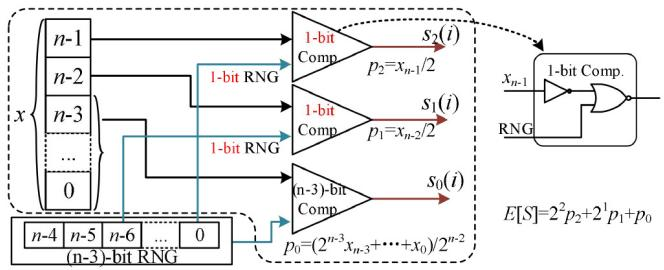
\includegraphics[width=0.48\linewidth]{images/903e64a4fe457b22a312a07e590d643ededfadda1d09e988113186457165d69e.jpg}
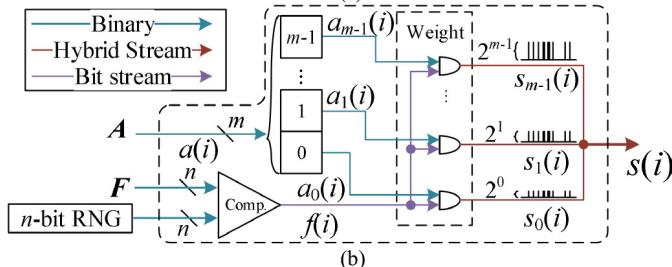
\includegraphics[width=0.48\linewidth]{images/9802c3ac18121324fe2a439263a2c6b79adfff9d32dcaa8d4a4012077dbba27f.jpg}
\caption{混合逻辑计算的BN-SB转换器. (a)A型使用一个二进制数据编码3比特流. (b)B型使用两个二进制数据编码混合流. }
\label{fig:5}
\end{figure}

因此，BN-SB（A型）输出的3比特流期望与$x$成正比，实现了BN $x$的多比特流编码
\begin{equation}
\begin{aligned}
E[S] &= 2^2p_2 + 2^1p_1 + 2^0p_0 \\
&= (2^{n-1}x_{n-1} + 2^{n-2}x_{n-2} \ldots + x_0)/2^{n-2} = x/2^{n-2}.
\end{aligned}
\label{eq:8}
\end{equation}

B型电路如图\ref{fig:5}(b)所示，是另一种编码多比特流的方法，使用两个BN编码一个多比特流. 输出的多比特流表示两个输入BN的乘积. 待编码的BN $x$（$n+m$比特）为$y$与$p$的乘积，即$x = y \cdot p = y \cdot z/2^n$. 其中，$z$为$n$比特，$y$为$m$比特，且$p \in [0, 1)$. 通过$z$与随机数的比较生成表示$p$的比特流$f(i)$，这与传统SC的BN-SB电路相同
\begin{equation}
E[F] = p = z/2^n.
\label{eq:9}
\end{equation}

此后，若$a(i) = y$且$i = 1, 2, \ldots, N$，则$E[A] = y$. 

最后，将$a(i)$和$f(i)$相乘得到$s(i)$，如图\ref{fig:5}右侧所示. 其中，$a_0(i), a_1(i), \ldots, a_{m-1}(i)$表示$a(i)$的$m$比特. $s(i)$的$m$比特与$a(i)$具有相同的表示方式
\begin{equation}
s(i) = \sum_{j=0}^{m-1}2^js_j(i) = \sum_{j=0}^{m-1}2^j[a_j(i) \cdot f(i)].
\label{eq:10}
\end{equation}

$s(i)$表示的值由其期望决定. 因$A$为常数，由(11)可得期望. 因此，$s(i)$为表示$x$的多比特流，该电路实现了将BN $x$转换为多比特流的功能
\begin{equation}
E[S] = \left(\sum_{j=0}^{m-1}2^jy_j\right)E[F] = y \cdot E[F] = y \cdot p = x.
\label{eq:11}
\end{equation}

与传统比特流相比，混合逻辑计算对流长度$N$的要求更低即可达到相同的分辨率. 将$n$比特BN $x$转换为$(m+1)$比特流时，$(m+1)$比特流的每个比特流具有$(n-m)$比特分辨率$(N = 2^{n-m}-1)$，足以表示$x_i$；而经典SC需要$n$比特分辨率$(N = 2^n-1)$. 

当$m = 0$时，混合逻辑流退化为经典比特流. 这是一种极端情况，具有最低的硬件开销但最差的延迟. 当$m = n-1$时，混合逻辑流转换为BN. 这是另一种极端情况，具有最佳的延迟和最大的硬件开销. 通过这种混合逻辑，可在延迟与硬件开销之间进行权衡，而非仅限于两种极端情况之间的选择. 

\section{混合逻辑计算讨论}

\subsection{混合逻辑的噪声容限}

在噪声环境中，假设随机流的每个比特具有相同的比特翻转率$a \in [0, 0.5]$. 此外，比特流$x(i)$由离散随机变量$X$生成，$X$的期望为$p \in [0, 1]$. $X_{\text{noise}}$表示受噪声影响的随机变量. $x(i)$比特翻转的四种情况如下：
\begin{enumerate}
    \item 发送1得到1，$p_1 = p(1-a)$
    \item 发送1得到0，$p_2 = pa$
    \item 发送0得到1，$p_3 = (1-p)a$
    \item 发送0得到0，$p_4 = (1-p)(1-a)$. 
\end{enumerate}

由此可得$X_{\text{noise}}$的期望：
\begin{equation}
E[X_{\text{noise}}] = p_1 + 0 \cdot p_2 + p_3 + 0 \cdot p_4 = (1-2a)E[X] + a.
\label{eq:12}
\end{equation}

SC的特性表明，$X_{\text{noise}}$的期望与$X$之间存在确定的线性关系，该关系与比特翻转率$a$相关. 该特性使SC具有高噪声容限. 需要注意的是，当$a = 0.5$时，$E[X_{\text{noise}}] = 0.5$，此时$X_{\text{noise}}$与$X$无关，信息完全丢失. 

$m$比特流$s(i)$可视为比特流$s_0(i), \ldots, s_{m-1}(i)$的并行组合，且(13)亦适用于$s_0(i), \ldots, s_{m-1}(i)$. 假设随机流的每个比特具有相同的比特翻转率$a$，且$E[S_i] = p_i, i = 0, 1, \ldots, m-1$. $s$的期望为
\begin{equation}
E[S] = 2^{m-1}E[S_{m-1}] + 2^{m-2}E[S_{m-2}] + \ldots + 2^0E[S_0].
\label{eq:13}
\end{equation}

由(12)和(13)可得，受噪声影响的$m$比特流$s(i)$的期望如(14)所示. 比特翻转误差同样导致混合流期望的线性变化，便于恢复原始数据. 因此，混合流具有与比特流相同的噪声容限. HSC基于比特流、多比特流和二进制数据的噪声容限如图\ref{fig:6}所示. 

\begin{figure}[htbp]
\centering
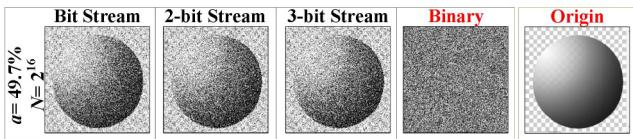
\includegraphics[width=0.8\linewidth]{images/ae20d6c0fca54d2c87470fff069626b7fb84e96feead0d3a84c1a7da79c663dc.jpg}
\caption{HSC噪声容限实验}
\label{fig:6}
\end{figure}

\begin{equation}
\begin{aligned}
E[S_{\text{noise}}] &= 2^{m-1}E[S_{m-1,\text{noise}}] + \ldots + 2^0E[S_{0,\text{noise}}] \\
&= (1-2a)(2^{m-1}p_{m-1} + \ldots + 2^0p_0) + a(2^{m-1} + \ldots + 2^0) \\
&= (1-2a)E[S] + a(2^m-1).
\end{aligned}
\label{eq:14}
\end{equation}

\subsection{混合逻辑的精度实验}

渐进精度[16]的存在使得通过选择不同流长度即可灵活调整精度，这是SC的优点之一. 由于真RNG的硬件实现较为复杂，SC中通常使用伪随机序列. 使用伪随机序列时，通过统计方法获得渐进精度是更优策略，以下测试均采用该策略. 

\begin{figure}[htbp]
\centering
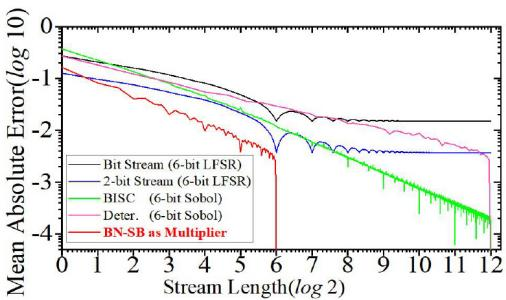
\includegraphics[width=0.8\linewidth]{images/cdc9458e92d66e73e5161320b8eff405bbeea64614388f229a782c4895f70840.jpg}
\caption{经典SC[1]、BISC[7]、确定性方法[15]、2比特流和HSC的BN-SB的MAE}
\label{fig:7}
\end{figure}

以二进制计算为基准，计算SC与BN之间乘法的偏差. 平均绝对误差（MAE）用作精度指标（MAE越低表示精度越高）. $SC(A,B,N)$表示流长度$N$下$A \times B$的SC结果，$P(A,B)$表示$A \times B$的理论值，其中$A$为$n$比特，$B$为$m$比特. 当$\text{MAE}(N) = 0$时，SC结果与BN计算完全一致，表明实现了零误差计算[15]
\begin{equation}
\text{MAE}(N) = \frac{\sum_{A=0}^{2^n-1}\sum_{B=0}^{2^m-1}|SC(A,B,N) - P(A,B)|}{2^{n+m}}.
\label{eq:15}
\end{equation}

图\ref{fig:7}展示了使用不同RNG执行6比特乘法时四种方法的MAE. 在比特流方法中，包括经典方法[1]、二进制接口SC（BISC）[7]和确定性方法的时钟分频[15]，其中BISC具有最佳的渐进精度. BN-SB实现零误差计算的速度比确定性方法快$2^6$倍. 当$N < 2^6$时，2比特流方法的MAE优于比特流方法. 

\begin{table*}[htbp]
\centering
\caption{三种方法的延迟(N)、面积、功耗和效率}
\label{tab:1}
\begin{tabular}{cccccccccc}
\toprule
\multicolumn{3}{c}{逻辑类型} & \multicolumn{3}{c}{比特流} & \multicolumn{2}{c}{混合流} & \multirow{3}{*}{二进制} \\
\cmidrule(lr){1-3}\cmidrule(lr){4-6}\cmidrule(lr){7-8}
\multicolumn{3}{c}{方法} & [1] & [7] & [15] & 图\ref{fig:2} & BN-SB &  \\
\cmidrule(lr){1-3}\cmidrule(lr){4-6}\cmidrule(lr){7-8}
\multicolumn{3}{c}{RNG (n比特)} & LFSR & Sobol & Sobol & LFSR & Sobol &  \\
\midrule
\multirow{6}{*}{\begin{tabular}[c]{@{}c@{}}比特宽度\\(n比特)\end{tabular}} &
\multirow{2}{*}{4} & MAE & 0.03 & 0.03 & 0.03 & 0.03 & 0.03 & 0 \\
 & & N & 16 & 17 & 81 & 9 & 6 & 1 \\
\cmidrule(lr){2-9}
 & \multirow{2}{*}{6} & MAE & 0.017 & 0.017 & 0.016 & 0.017 & 0.016 & 0 \\
 & & N & 64 & 46 & 169 & 39 & 12 & 1 \\
\cmidrule(lr){2-9}
 & \multirow{2}{*}{8} & MAE & 0.008 & 0.008 & 0.008 & 0.008 & 0.008 & 0 \\
 & & N & 256 & 122 & 576 & 169 & 24 & 1 \\
\midrule
\multirow{2}{*}{面积 (n=8)} & \multicolumn{2}{c}{LUT} & 18 & 29 & 20 & 20 & 17 & 64 \\
 & \multicolumn{2}{c}{FF} & 32 & 40 & 32 & 32 & 24 & 48 \\
\midrule
\multicolumn{3}{c}{$*(\times 10^{-4})$, n=8} & 2.17 & 2.8 & 0.87 & 2.95 & 24.5 & 156.3 \\
\midrule
\multicolumn{3}{c}{功耗(W) (n=8, 600 MHz)} & 0.009 & 0.01 & 0.009 & 0.008 & 0.007 & 0.018 \\
\midrule
\multicolumn{3}{c}{$**$(OPS/W)$(\times 10^9)$} & 0.26 & 0.49 & 0.12 & 0.44 & 3.57 & 33.3 \\
\bottomrule
\multicolumn{9}{l}{$*$面积效率$=(\text{LUT} \times N)^{-1}$，$N$是流长度，表示延迟. } \\
\multicolumn{9}{l}{$**$能耗效率$=600\text{ MHz}/(N \cdot \text{功率})$，n=8比特，OPS表示每秒乘法操作数. } \\
\end{tabular}
\end{table*}

表\ref{tab:1}对比了混合逻辑计算与传统SC达到相同精度所需的延迟，采用MAE测量误差. 如[8]所述，由于生成的比特流存在重复，经典方法[1]的精度在流长度$N > 2^n$后不再提高. 因此，测试中的流长度$N$亦不超过$2^n$. 基于经典SC在不同比特宽度BN上操作所达到的最佳精度，测试了其他方法达到相同精度所需的流长度. 

使用Kintex-7 FPGA（现场可编程门阵列）实现了具有8比特数据输入的不同方法电路，所有数据均来自设计工具，如表\ref{tab:1}所示. 计算$(\text{LUT} \times N)^{-1}$以测量各方法的面积效率. BN-SB作为乘法器和BISC均存在局限性，仅适用于多项式操作的第一次乘法，或需将随机流输出转换为BN后方可进行下一次乘法. BN-SB作为乘法器的面积效率是测试中所有方法中最优的，达到经典SC方法的11.3倍. 2比特混合流与BISC的面积效率相近，相较于经典SC提高了约30\%. 

\section{结论}

本文提出了一种称为HSC的新数据表示方法. 该方法利用多比特流的期望实现SC. 与传统SB相比，混合逻辑计算实现了低延迟和低面积占用，克服了经典方法的长延迟问题. 文中论证了多比特流计算规则的合理性，并设计了HSC的基本电路. 在精度实验中，使用BN-SB作为乘法器将延迟降低至$1/2^m$以达到零误差计算. 使用8比特输入数据时，BN-SB作为乘法器的面积效率达到经典SC方法的11.3倍. 

\begin{thebibliography}{17}

\bibitem{1}
B. R. Gaines, ``Stochastic computing systems,'' in \textit{Advances in Information Systems Science}, Boston, MA, USA: Springer, 1969, pp. 37--172.

\bibitem{2}
A. Alaghi and J. Hayes, ``Survey of stochastic computing,'' \textit{ACM Trans. Embedded Comput. Syst.}, vol. 12, no. 2s, p. 92, 2013.

\bibitem{3}
T. Moreau et al., ``A taxonomy of general purpose approximate computing techniques,'' \textit{IEEE Embedded Syst. Lett.}, vol. 10, no. 1, pp. 2--5, Mar. 2018.

\bibitem{4}
P. Li, D. J. Lilja, W. Qian, K. Bazargan, and M. D. Riedel, ``Computation on stochastic bit streams digital image processing case studies,'' \textit{IEEE Trans. Very Large Scale Integr. (VLSI) Syst.}, vol. 22, no. 3, pp. 449--462, Mar. 2014.

\bibitem{5}
K. Han, J. Wang, and W. J. Gross, ``Bit-wise iterative decoding of polar codes using stochastic computing,'' in \textit{Proc. Great Lakes Symp. VLSI (GLSVLSI)}, 2018, pp. 409--414.

\bibitem{6}
S. Sato, K. Nemoto, S. Akimoto, M. Kinjo, and K. Nakajima, ``Implementation of a new neurochip using stochastic logic,'' \textit{IEEE Trans. Neural Netw.}, vol. 14, no. 5, pp. 1122--1127, Sep. 2003.

\bibitem{7}
H. Sim, D. Nguyen, J. Lee, and K. Choi, ``Scalable stochastic-computing accelerator for convolutional neural networks,'' in \textit{Proc. 22nd Asia South Pacific Des. Auto. Conf. (ASP-DAC)}, Jan. 2017, pp. 696--701.

\bibitem{8}
M. H. Najafi and D. J. Lilja, ``High quality down-sampling for deterministic approaches to stochastic computing,'' \textit{IEEE Trans. Emerg. Topics Comput.}, vol. 9, no. 1, pp. 7--14, Jan.-Mar. 2021.

\bibitem{9}
K. K. Parhi, ``Analysis of stochastic logic circuits in unipolar, bipolar and hybrid formats,'' in \textit{Proc. IEEE Int. Symp. Circuits Syst. (ISCAS)}, 2017, pp. 1--4.

\bibitem{10}
S. Liu and J. Han, ``Toward energy-efficient stochastic circuits using parallel sobol sequences,'' \textit{IEEE Trans. Very Large Scale Integr. (VLSI) Syst.}, vol. 26, no. 7, pp. 1326--1339, Jul. 2018.

\bibitem{11}
V. Canals, A. Morro, A. Oliver, M. L. Alomar, and J. L. Rossell\'{o}, ``A new stochastic computing methodology for efficient neural network implementation,'' \textit{IEEE Trans. Neural Netw. Learn. Syst.}, vol. 27, no. 3, pp. 551--564, Mar. 2016.

\bibitem{12}
A. Ardakani, F. Leduc-Primeau, N. Onizawa, T. Hanyu, and W. Gross, ``VLSI implementation of deep neural network using integral stochastic computing,'' \textit{IEEE Trans. Very Large Scale Integr. (VLSI) Syst.}, vol. 25, no. 10, pp. 2688--2699, Oct. 2017.

\bibitem{13}
M. H. Najafi, S. R. Faraji, B. Li, D. J. Lilja, and K. Bazargan, ``Accelerating deterministic bit-stream computing with resolution splitting,'' in \textit{Proc. 20th Int. Symp. Qual. Electron. Des. (ISQED)}, 2019, pp. 157--162.

\bibitem{14}
S. R. Faraji and K. Bazargan, ``Hybrid binary-unary hardware accelerator,'' \textit{IEEE Trans. Comput.}, vol. 69, no. 9, pp. 1308--1319, Sep. 2020.

\bibitem{15}
M. H. Najafi, D. Jenson, J. Lilja, and D. Riedel, ``Performing stochastic computation deterministically,'' \textit{IEEE Trans. Very Large Scale Integr. (VLSI) Syst.}, vol. 27, no. 12, pp. 2925--2938, Dec. 2019.

\bibitem{16}
A. Alaghi and J. P. Hayes, ``Fast and accurate computation using stochastic circuits,'' in \textit{Proc. Des. Automat. Test Eur. Conf. Exhib. (DATE)}, 2014, pp. 1--4.

\bibitem{17}
Y. Chen and H. Li, ``Novel stochastic computing using amplitude and frequency pulse encoding,'' in \textit{Proc. IEEE Int. Symp. Circuits Syst. (ISCAS)}, 2022, pp. 656--660.

\end{thebibliography}

\end{document}
